\section{SEDflow} \label{sec:sedflow}
In this work we apply ANPE to SED modeling of galaxy spectra. 
tl;dr of intro 

% section explaining specific SED set up 
\subsection{SED Modeling: PROVABGS} \label{sec:provabgs}
To model SEDs, we use the state-of-the-art stellar population synthesis (SPS)
model of the PROVABGS~(\chedit{Hahn~\etal~2022}). 
With SPS modeling, we model the SED of a galaxy a as a composite of stellar
populations defined by stellar evolution theory (in the form of isochrones,
stellar spectral libraries, and an initial mass function) and its star
formation and chemical enrichment histories (SFH and ZH), attenuated by
dust~\citep[see][for a review]{conroy2013}. 
The PROVABGS model, in particular, utilizes a non-parametric SFH with a
starburst, a non-parametric ZH that varies with time, and a flexible dust
attenuation prescription.

% highlight advantages of provabgs 
The SFH has two components: one based on non-negative matrix factorization
(NMF) bases and the other, a starburst component.
The SFH contribution from the NMF component is a linear combination of four NMF
SFH basis functions, that are derived from performing NMF~\citep{lee1999,
cichocki2009, fevotte2011}
on smoothed SFHs of simulated galaxiese of the Illustris cosmological
hydrodyanmic simulations~\citep{vogelsberger2014, genel2014, nelson2015}.
The NMF SFH prescription provides a compact and flexible representation of the
SFH, assuming that the SFHs of Illustris galaxies resemble the SFHs of real
galaxies. 
To add stochasticity to the SFH, we include a second star burst component that
consists of a single stellar population (SSP). 

The ZH is similar defined using two NMF bases dervied from Illustris ZHs. 
Most SPS models assume constant metallicity over
time~\citep[\emph{e.g.}][]{carnall2017, leja2019}; however, this assumption can
significantly bias inferred galaxy properties~\citep{thorne2021}. 
Instead by using the NMF prescription, we can flexibly model a range of
different ZHs with only two extra parameters.  
The stellar evolution theory is based on Flexible Stellar Population
Synthesis~\citep[FSPS;][]{conroy2009, conroy2010c} with the MIST
isochrones~\citep{paxton2011, paxton2013, paxton2015, choi2016, dotter2016},  
the \cite{chabrier2003} initial mass function (IMF), and a combination of the
MILES~\citep{sanchez-blazquez2006} and BaSeL~\citep{lejeune1997, lejeune1998,
westera2002} libraries.
The SFH and ZH are binned into 43 logarithmically-space time bin and SSPs are
evalulated at each time bin using FSPS. 
The SSPs are summed up to get the unattenuated rest-frame galaxy SED. 

Finally, PROVABGS attenuates the light from the composite stellar population
using the two component \cite{charlot2000} dust attenuation model with
diffuse-dust (ISM) and birth cloud (BC) components. 
All SSPs are attenuated by the diffuse dust using the \cite{kriek2013}
attenuation curve.
Then, the BC component provides extra dust attenuation on SSPs younger than 100
Myr with young stars that are embedded in modecular clouds and HII regions. 
In total the PROVABGS SED model has 12 free parameters: stellar mass ($M_*$),
six SFH parameters ($\beta_1, \beta_2, \beta_3, \beta_4, t_{\rm burst}, f_{\rm
burst}$), two ZH parameters ($\gamma_1, \gamma2$), and three dust attenuation
parameters ($\tau_{\rm BC}, \tau_{\rm ISM}, n_{\rm dust}$). 
Each PROVABGS model evaluation takes \chedit{X} seconds. 


\begin{figure}
\begin{center}
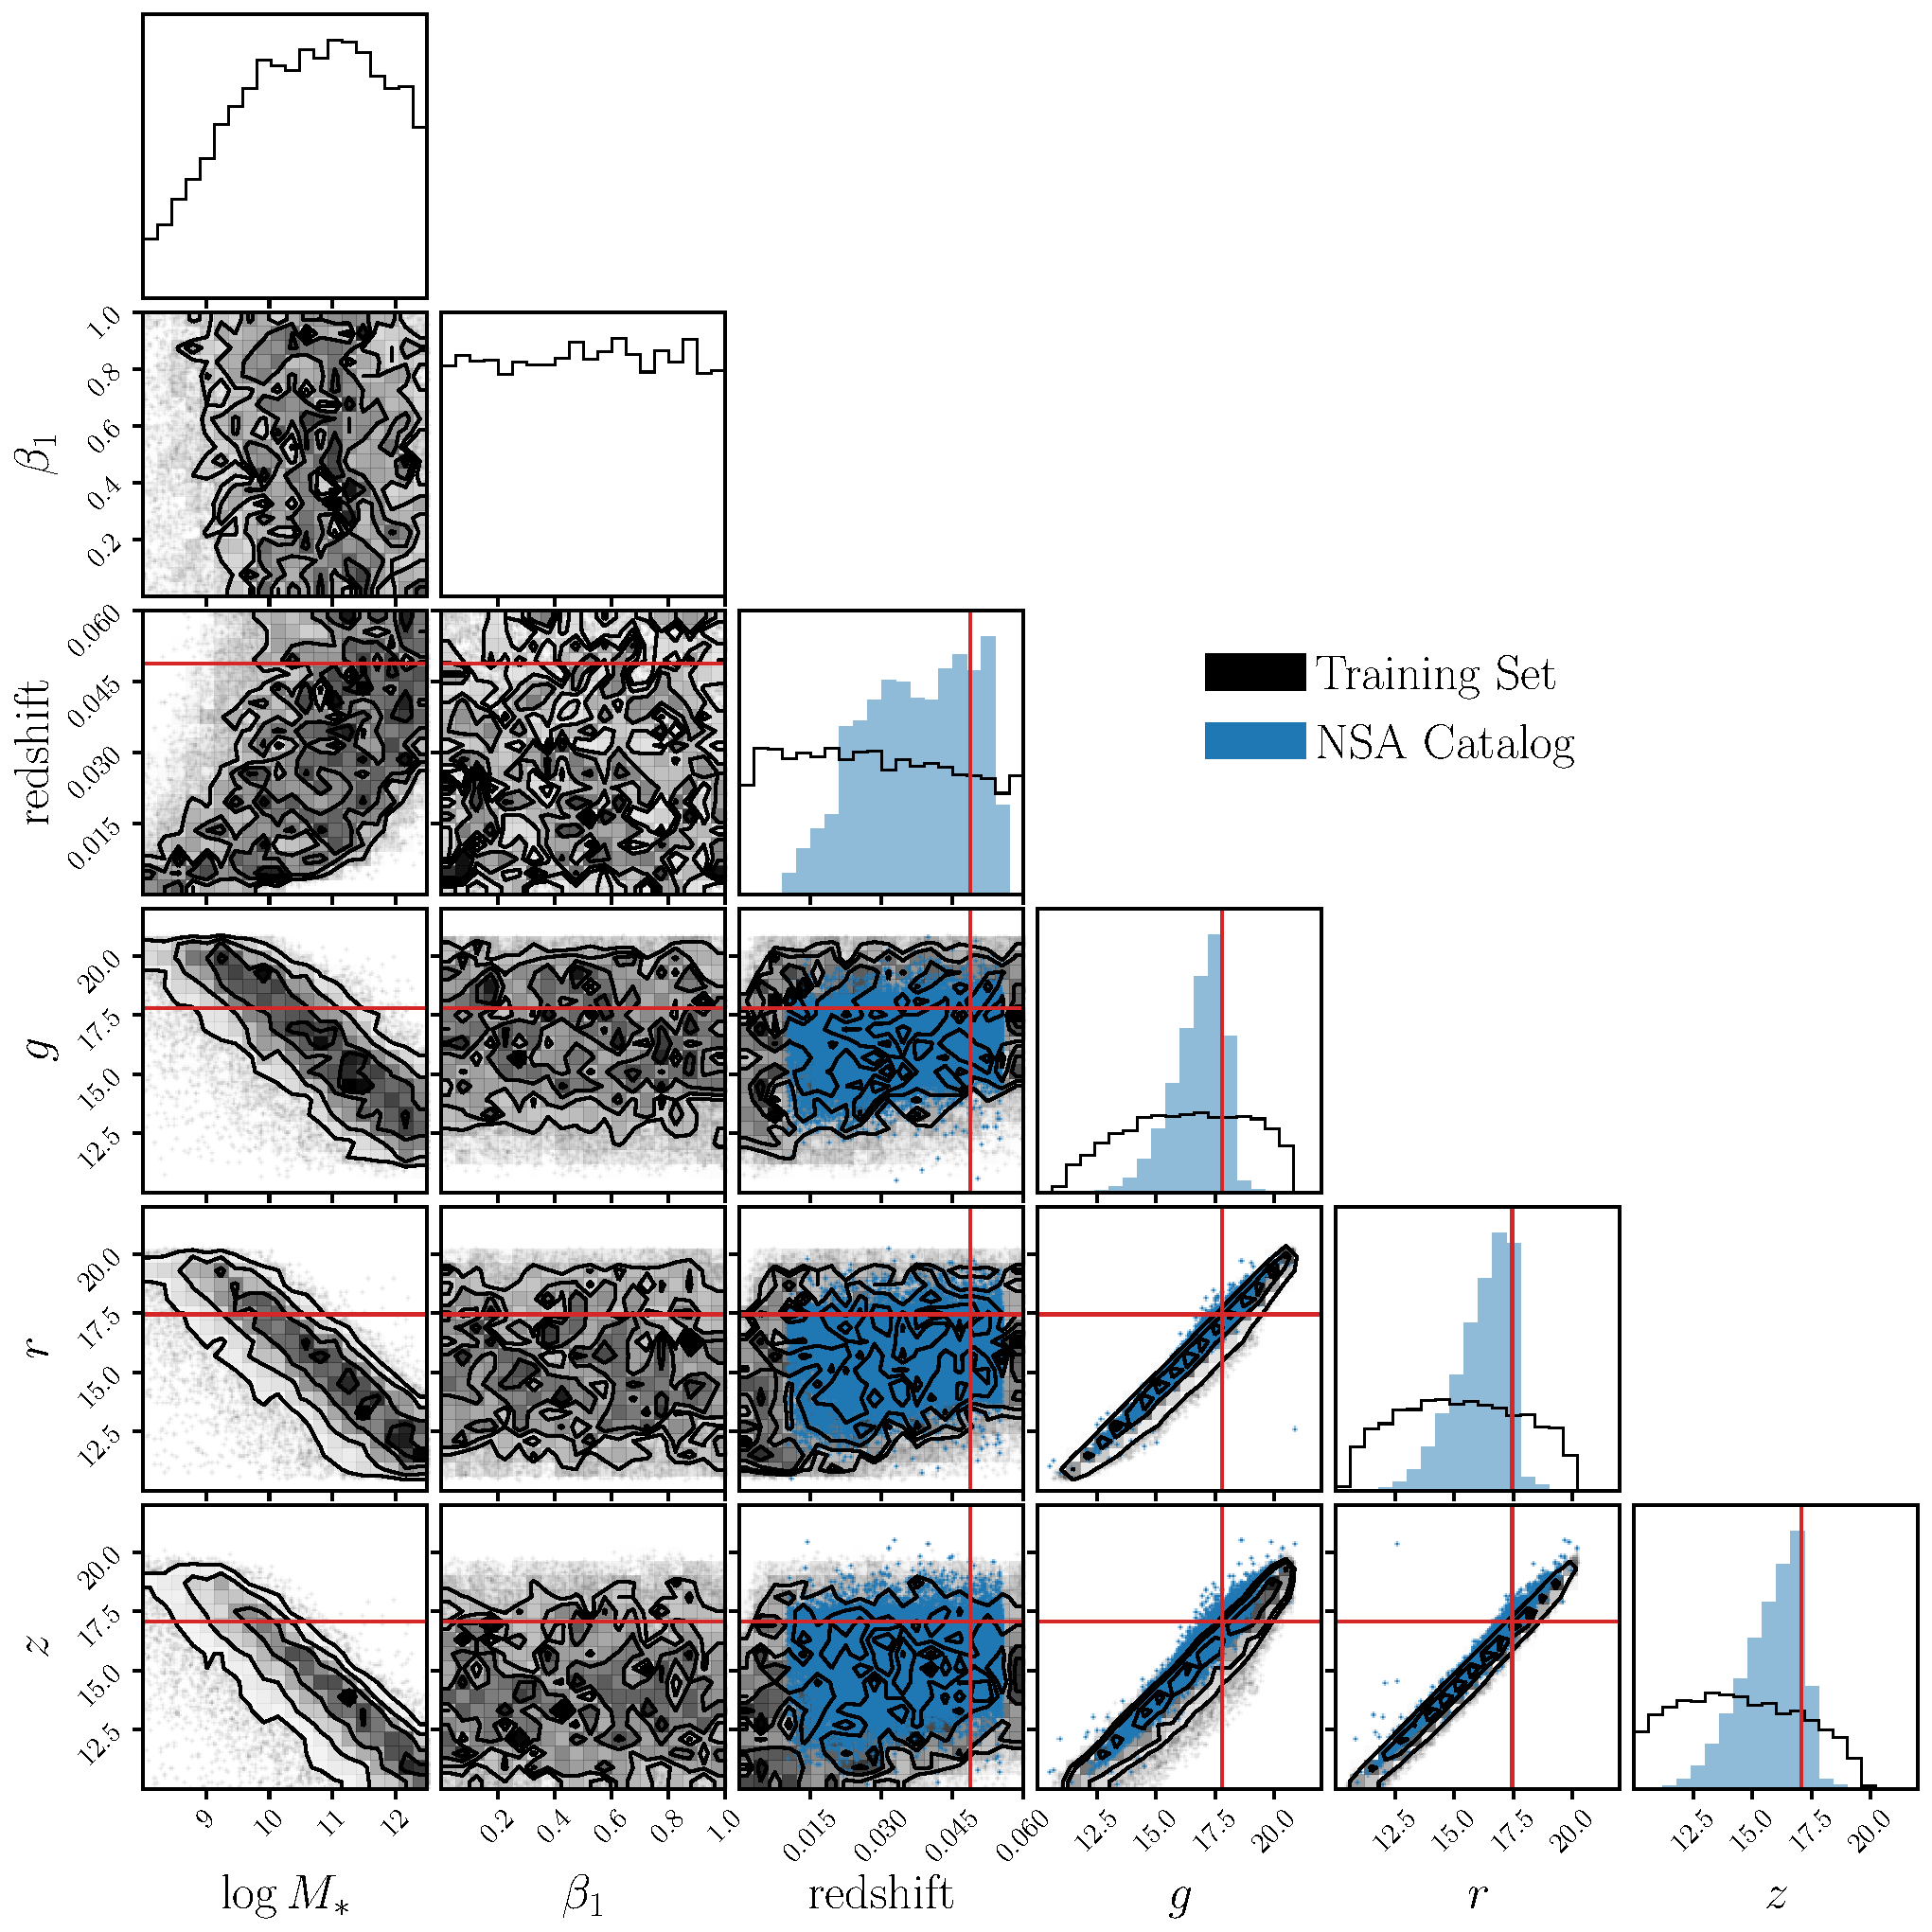
\includegraphics[width=0.9\textwidth]{figs/training.pdf}
    \caption{\label{fig:data}
    Joint distribution of SED model parameters ($\log M_*$, $\beta_1$,
    redshift) and photometric magnitudes ($g$, $r$, $z$) for our training set.
    The training set was constructed by sampling parameter values from the
    prior, constructing SEDs using a theoretical SPS
    model, and applying our noise model. 
    For details, we refer readers to Section~\ref{sec:sedflow}.
    For comparison, we present the distribution of magnitudes for galaxies in
    the NSA catalog (blue). 
    \emph{The training set fully encompasses the observations, thus, our 
    {\sc SEDflow} method can be used to infer the posterior for all NSA
    galaxies}.
    }
\end{center}
\end{figure}
%%%%%%%%%%%%%%%%%%%%%%%%%%%%%%%%%%%%%%%%%%%%%%%%%%%%%%%%%%%%%%%%%%%%%%%%%%%%
% training data 
%%%%%%%%%%%%%%%%%%%%%%%%%%%%%%%%%%%%%%%%%%%%%%%%%%%%%%%%%%%%%%%%%%%%%%%%%%%%
\subsection{Training Data} \label{sec:training}
In this section, we describe how to we construct the training data using our
SED model.
First, we sample $N_{\rm train}$ SED model parameters from a prior: $\theta'\sim p(\theta)$. 
We use the same priors as \chedit{Hahn \etal~(2022)}: uniform priors over $M_*,
t_{\rm burst}, f_{\rm burst}, \gamma_1, \gamma2, \tau_{\rm BC}, \tau_{\rm ISM},
n_{\rm dust}$ and Dirichlet prior over $\beta_1, \beta_2, \beta_3, \beta_4$. 
The Dirichlet prior is chosen for the normalization of the NMF SFH while the
rest are chosen to span an extensive range of galaxy SEDs. 

For each sampled SED parameters, we construct mock observables --- \emph{i.e.}
NSA optical photometry (Section~\ref{sec:obs}) --- 
We first construct the rest-frame galaxy SED using the SED model,
$F(\lambda;\theta')$. 
Then, for a given redshift, $z$, we redshift the SED and convolve it with
optical broadband filters, $R_X$ to generate noiseless photometric fluxes:
\begin{equation}
    f_X(\theta') = \int F(\lambda;\theta') \, R_X(\lambda) \, {\rm d}\lambda
\end{equation}
Next, we apply a noise model.

In our noise model, we first assign photometric uncertainties, $\sigma'_X$, to
the training data by sampling an estimate of $p(\sigma_X | f_X)$. 
Then, we apply Gaussian noise
\begin{equation}
    \hat{f}_X(\theta') = f_X(\theta') + n_X  \quad {\rm where}~n_X \sim \mathcal{N}(0, \sigma'_X)
\end{equation}
to derive photometric flux.
We emphasize that the accuracy of the posteriors from our ANPE is not
particularly sensitive to the noise model. 
This is because $\sigma_X$ is included in the conditional statement of our
posterior. 
Hence,  we only require that $\sigma'_X$ of the training data spans the observed
$\sigma_X$ values. 
We discuss this further in Section~\ref{sec:discuss}.

Since we do not require a high fidelity estimate of $p(\sigma_X | f_X)$, we use
a simple empirical estimate of $p(\sigma_X | f_X)$ based on NSA photometry and
uncertainties. 
For each band, we separately estimate  
\begin{equation}
    \hat{p}(\sigma_X | f_X) = \mathcal{N}( \mu_{\sigma_X}(f_X), \sigma_{\sigma_X}(f_X))
\end{equation}
as a Gaussian in magnitude-space. 
$\mu_{\sigma_X}$ and $\sigma_{\sigma_X}$ are the median and standard deviation
of $\sigma_X$ as a function of $f_X$ that we estimate by evaluating them in
$f_X$ bin and interpolating over the bins. 
Any $\theta'$ that is assigned a negative $\sigma'_X$ is removed from our
training data. 
We also remove any training data with $f_X(\theta'$ outside the range of NSA
photometry. 

In total, we constuct $N_{\rm train} = 1,131,561$ sets of SED parameters,
redshift, photometric uncertainty, and mock NSA photometry: 
$\{(\theta', z, \sigma'_X, \hat{f}_X(\theta') \}$.
There are 12 SED parameters and photometry and uncertainties in each of the 5
NSA bands. 
In Figure~\ref{fig:data}, we present the joint distribution of select SED model
parameters ($\log M_*$, $\beta_1$), redshift, photometry ($g$ and $r$ bands),
and photometric uncertainty ($r$ band) of our training data (black).
We also include the distribution of redshift, photometry, and uncertainty of
NSA galaxies (blue).
The photometry and uncertainties are in magnitude-space. 
The distribution of the training data fully spans the distribution of NSA
galaxies.
Hence, the training data provides support over the full $(f_X, \sigma_X, z)$
space of the NSA observations and the trained ANPE can accurately estimate
posteriors for all NSA galaxies. 

\subsection{Training ANPE} \label{sec:anpe}
description of the ANPE training
\begin{itemize}
    \item architecture
    \item validation 
\end{itemize}
